Разработанные алгоритмы также можно протранслировать и для расчета трехкристальных спектров дифракции.
В простейшем случае, когда все три кристалла находятся в точном положении брэгговской дифракции, рассчитать
интенсивность отраженного ими излучения не составляет труда.
На кристалл монохроматор (M) падает расходящийся набор рентгеновских лучей, каждый из которых характеризуется отстройкой
$\vartheta$ от точного брэгговского направления (рис. \ref{ris:triple_crystal_schem}). Отраженный луч с интенсивностью
$I_0 P_M(\vartheta)$ падает на образец и дальше, с интенсивностью $I_0 P_M(\vartheta)P_S(\vartheta)$,
  на анализатор интенсивность пучка после которого составляет $I_0 P_M(\vartheta)P_S(\vartheta)P_A(\vartheta)$.

Для более общего случая, когда кристаллы образца и анализатора отстроены на некоторые углы относительно
брэгговского (такая ситуация возникает постоянно в процессе измерений).
Необходимо также ввести угловые отстройки от точного брэгговского положения
для образца (S) $\theta$ и анализатора (A) $\varepsilon$.
В результате поворота образца на угол  $\theta$ относительно Брэгговского положения,
излучение отраженное от монохроматора, падает на образец
под углом $\theta_B+\theta+\vartheta$. Если кристалл повернуть на угол $\theta$,
 отраженный луч повернется на удвоенный угол
$2\theta$, в итоге излучение падает на анализатор (А) под углом $\theta_B+2\theta-\varepsilon+\vartheta$ (рис. \ref{ris:triple_crystal_schem}) \cite{trd_Bushuev_1997}.
\begin{figure}[H]
  \centering
  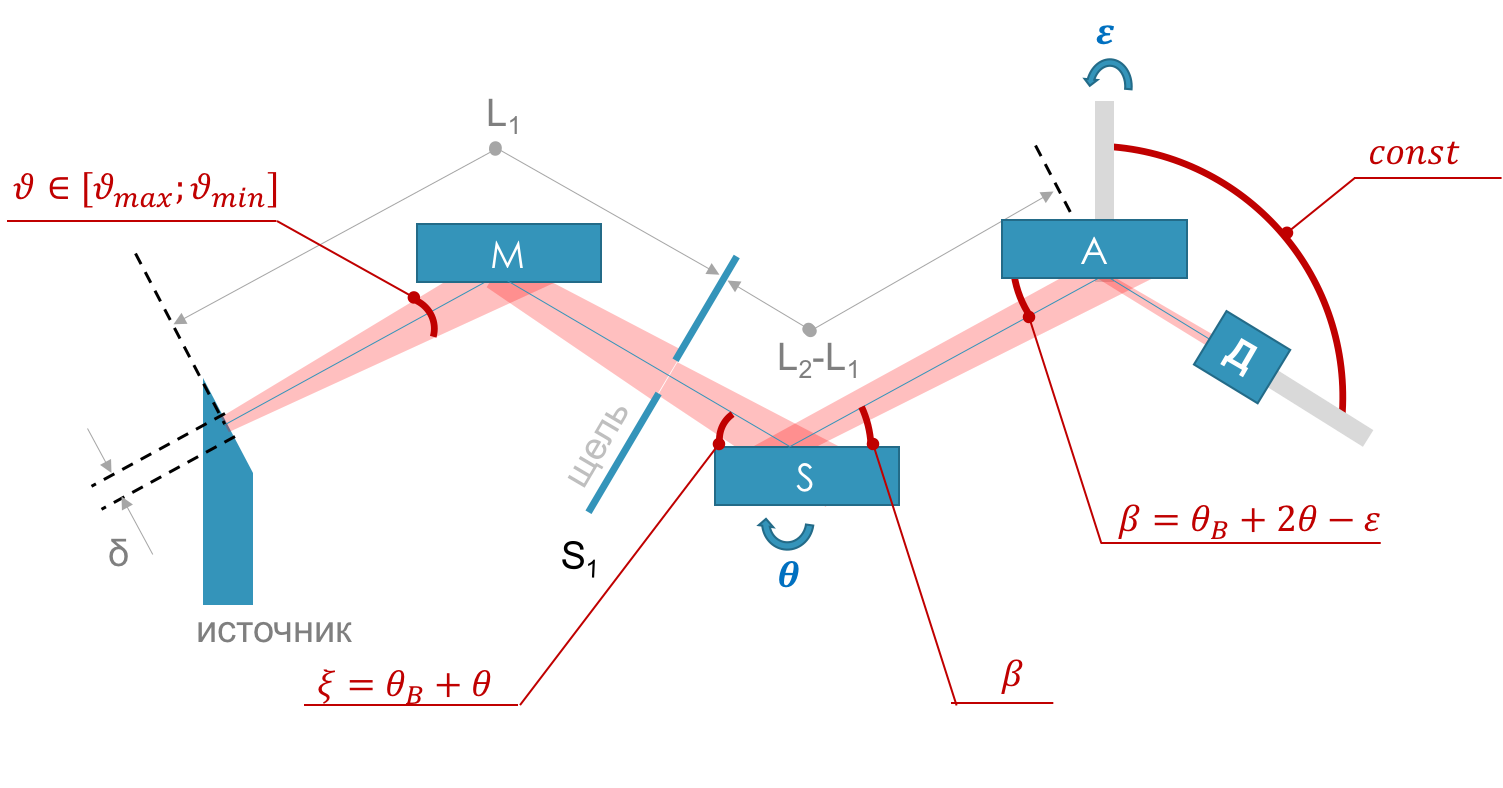
\includegraphics[width=0.8\textwidth]{images/triple_crystal_schem.png}
  \caption{Схема трехкристального эксперимента, $\theta$ - угловая отстройка образца от точного угла Брэгга,
  $\varepsilon$ - угол отстройки анализатора относительно положения оптической оси}
  \label{ris:triple_crystal_schem}
\end{figure}

% Учитывая что рентгеновская трубка имеет полихроматический спектр, лучи падающие под разными углами могут отражаться
% с одинаковым коэффициентом отражения за счет разной энергии $\frac{\lambda - \lambda_1}{\lambda_1}\tan(\theta_B)$,
Спектрально-угловое распределение, исходя из вышесказанного, задается выражением:

\begin{eqnarray} \label{eq:triplr_spectra_angle_map}
  P_{triple}(\vartheta,\lambda,\theta,\varepsilon) =I_0\cdot
    P_M \left(\vartheta - \frac{\lambda - \lambda_1}{\lambda_1}\tan(\theta_B) \right) \cdot \nonumber \\
   P_S \left(\theta + \vartheta - \frac{\lambda - \lambda_1}{\lambda_1}\tan(\theta_B)\right)  \cdot  \nonumber \\
   P_A \left(2\theta - \varepsilon + \vartheta - \frac{\lambda - \lambda_1}{\lambda_1}\tan(\theta_B)\right) \Bigg].
 \end{eqnarray}

  \begin{figure}[H]
    \centering
    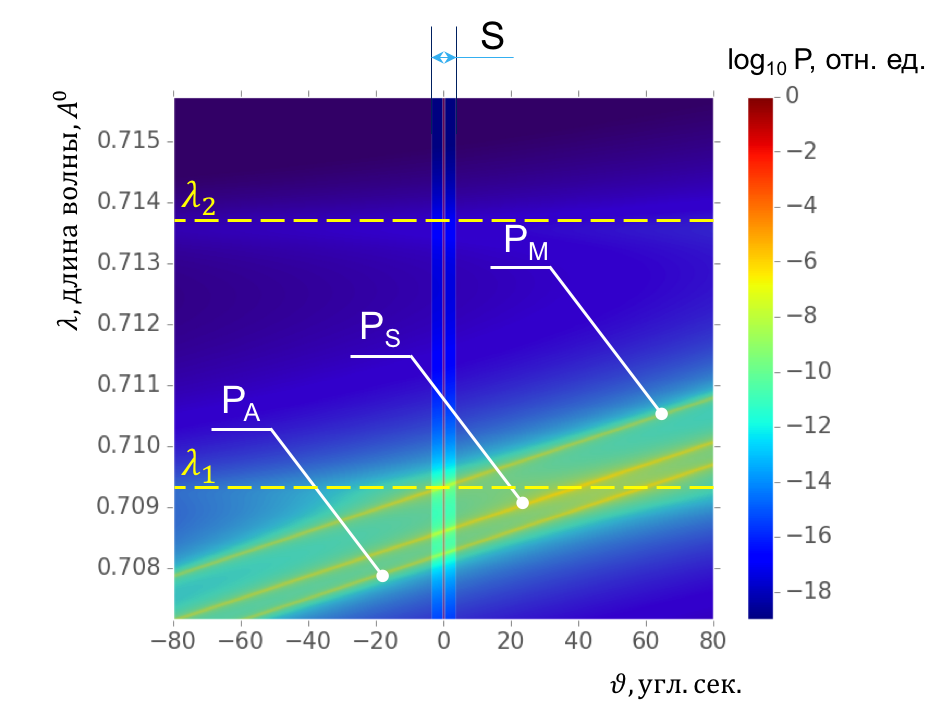
\includegraphics[width=0.6\textwidth]{images/triple_map.png}
    \caption{Спектрально-угловое распределение в случае трехосевой схемы
    для лабораторного источника с молибденовым анодом ($MoK_{\alpha}$).
    Образец отстроен на $\theta = - 50''$ относительно точного брэгговского положения,
    анализатора на $\varepsilon = 20''$ относительно
    зеркально отраженного луча после кристалла-образца. Так же на схеме изображено щелевое устройство размером около 7 $''$}
    \label{ris:triple_map}
  \end{figure}

Измерение карты обратного пространства производится путем комбинированного
сканирования по углам отстройки образца и анализатора.

Анализ поведения интегральной интенсивности, заключенной в пределах щели $S$,
в процессе такого сканирования позволяет сделать вывод о существовании трех
максимумов отражения. Каждый максимум возникает при таких комбинация углов отстройки
$\theta$ и $\varepsilon$, когд две из трех наклонных полосы отражения (монохроматора,
образца и анализатора) пересекаются в пределах полосы пропускания щели (см. рис. \ref{ris:triple_map_piks}).
Эти максимумы получили названия главного пика, псевдопика монохроматора и псевдопика анализатора.

\begin{figure}[H]
  \centering
  \subfloat[]{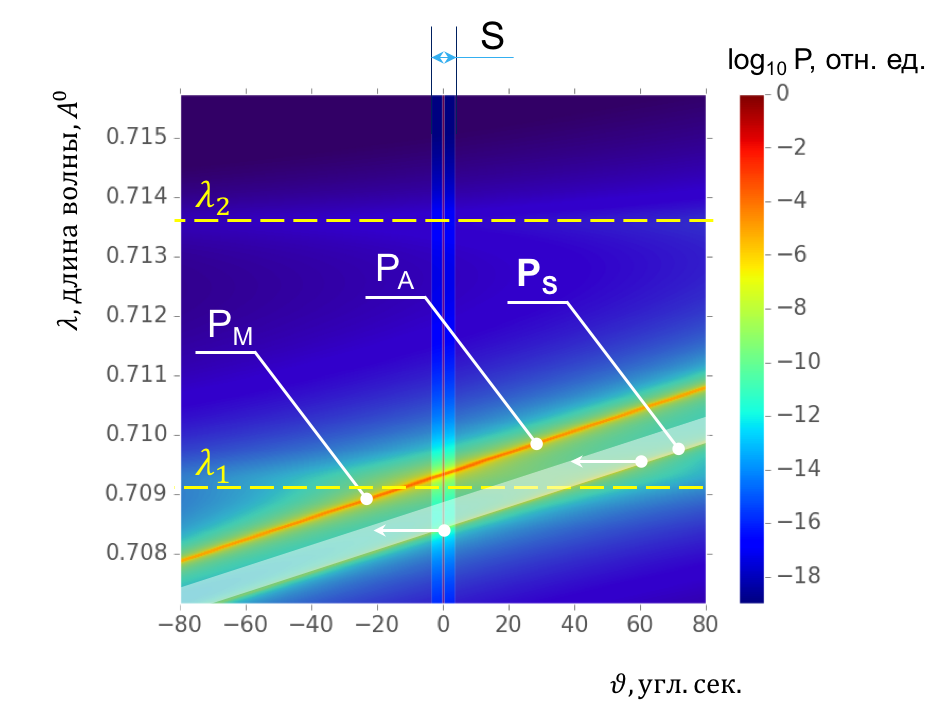
\includegraphics[width=0.32\textwidth]{images/triple_map_g.png}\label{ris:triple_map_piks_g}}
  \hfill
  \subfloat[]{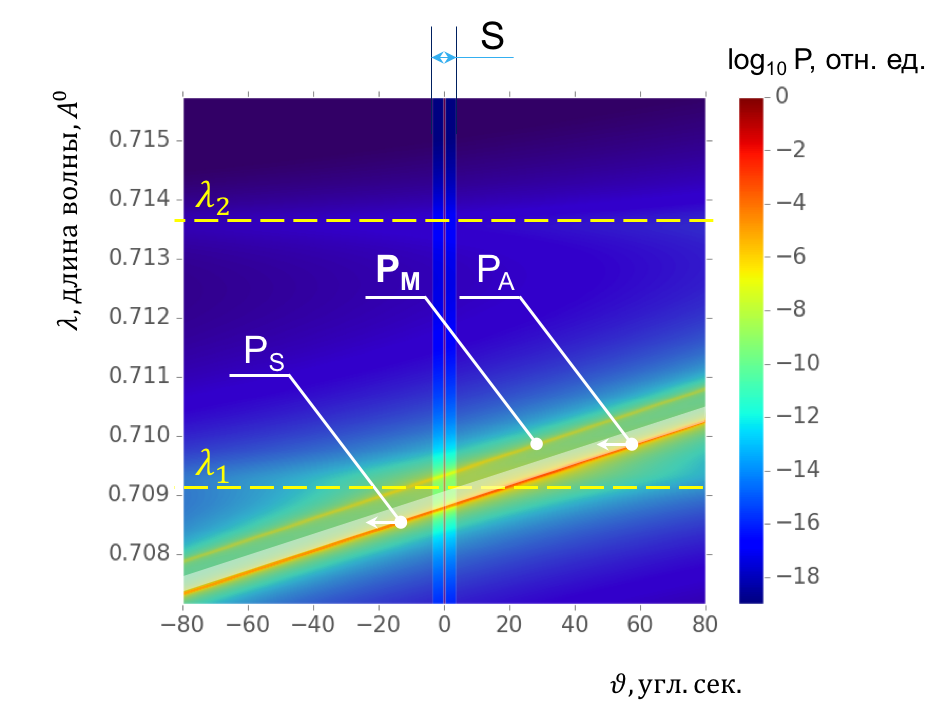
\includegraphics[width=0.32\textwidth]{images/triple_map_m.png} \label{ris:triple_map_piks_m}}
  \hfill
  \subfloat[]{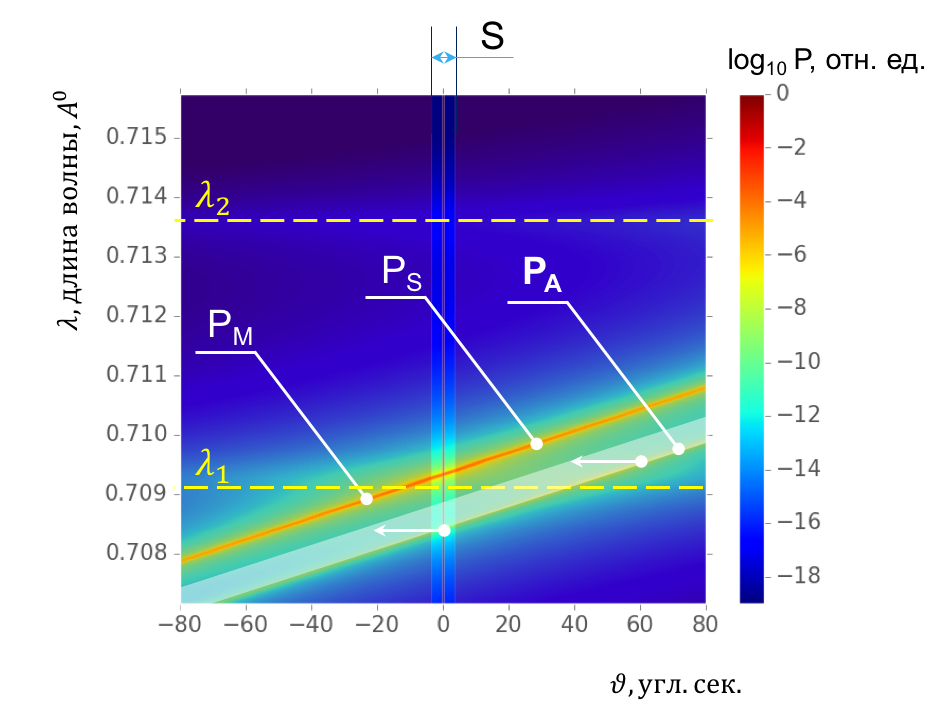
\includegraphics[width=0.32\textwidth]{images/triple_map_a.png} \label{ris:triple_map_piks_a}}
  \caption{Формирование карты рассеяния в прямом пространстве, вдоль направления главного пика (a),
  псевдопика монохроматора (b), псевдопика анализатора (c)}
  \label{ris:triple_map_piks}
\end{figure}

\subsubsection*{Главный пик}
Главный пик (ГП) формируется в случае отстройки кристалла-образца от точного угла Брэгга,
 и при повороте анализатора на $\varepsilon = 2\theta$, т.е. в том случае, когда
  образец поворачивается по отношению к падающему пучку в окрестности угла Брэгга,
  анализатор поворачивается таким образом, чтобы "ловить" дифрагированный пучок.
Тогда выражение (\ref{eq:triplr_spectra_angle_map}) примет частный вид:

\begin{eqnarray} \label{eq:triplr_spectra_angle_map_GP}
  P_{\text{ГП}}(\vartheta,\lambda,\theta,\varepsilon) =I_0\cdot
    P_M \left(\vartheta - \frac{\lambda - \lambda_1}{\lambda_1}\tan(\theta_B) \right) \cdot \nonumber \\
   P_S \left(\theta + \vartheta - \frac{\lambda - \lambda_1}{\lambda_1}\tan(\theta_B)\right)  \cdot  \nonumber \\
   P_A \left(0+\vartheta - \frac{\lambda - \lambda_1}{\lambda_1}\tan(\theta_B)\right) \Bigg].
 \end{eqnarray}

Как видно на рис. \ref{ris:triple_map_piks_g}, линия отражения анализатора и образца перекрывают друг друга и пик формируется
движением линии образца. Такой режим сканирования в экспериментальной практике называется $\theta-2\theta$ сканированием,
угол поворота образца соответствует удвоенному углу поворота анализатора. В этом случае детектором регистрируется чисто
зеркальная компонента отражения т.е., направляя на образец луч с фиксированными значениями отстройки $\vartheta$ и длины волны
 $\lambda$, анализируется отраженный луч с той же энергией и угловой составляющей.

\subsubsection*{Пседвопик монохроматора}
Псевдопик монохроматора (ППМ) (рис. \ref{ris:triple_map_piks_m}) формируется, когда линия отражения образца и анализатора
двигаются вместе, перекрываясь между собой. Угол отстройки образца и анализатора совпадает ($\theta = \varepsilon$).

\begin{eqnarray} \label{eq:triplr_spectra_angle_map_PPM}
  P_{\text{ППМ}}(\vartheta,\lambda,\theta,\varepsilon = \theta) =I_0\cdot
    P_M \left(\vartheta - \frac{\lambda - \lambda_1}{\lambda_1}\tan(\theta_B) \right) \cdot \nonumber \\
   P_S \left(\theta + \vartheta - \frac{\lambda - \lambda_1}{\lambda_1}\tan(\theta_B)\right)  \cdot  \nonumber \\
   P_A \left(\theta  + \vartheta - \frac{\lambda - \lambda_1}{\lambda_1}\tan(\theta_B)\right) \Bigg].
 \end{eqnarray}

 \subsubsection*{Пседвопик анализатора}
 Псевдопик анализатора (ППА) формируется, когда монохроматор и образец
 находятся в точном брэгговском положении, перекрываясь между собой. Движение вдоль ППА осуществляется
 движением линии отражения анализатора на карте спектрально-углового распределения (рис. \ref{ris:triple_map_piks_a}).
   Угол отстройки образца и анализатора совпадает ($\theta = 0$).

 \begin{eqnarray} \label{eq:triplr_spectra_angle_map_PPM}
   P_{\text{ППА}}(\vartheta,\lambda,\theta=0,\varepsilon) =I_0\cdot
     P_M \left(\vartheta - \frac{\lambda - \lambda_1}{\lambda_1}\tan(\theta_B) \right) \cdot \nonumber \\
    P_S \left(0 + \vartheta - \frac{\lambda - \lambda_1}{\lambda_1}\tan(\theta_B)\right)  \cdot  \nonumber \\
    P_A \left(0-\varepsilon  + \vartheta - \frac{\lambda - \lambda_1}{\lambda_1}\tan(\theta_B)\right) \Bigg].
  \end{eqnarray}


\subsubsection*{Интенсивность на детекторе}

Необходимо учитывать что детектирующее устройство фиксирует интегральную интенсивность в пределах аппертуры
щелевого коллиматора и по всем длинам волн.
Таким образом, общее выражение для интегральной интенсивности трехкратно отраженного
монохроматором, образцом и анализатором излучения рентгеновской трубки, попавшего в детектор через
щелевой коллиматор, в зависимости от углов отстройки от точного брэгговского положения образца $\theta$ и
анализатора $\varepsilon$ записывается в следующем виде:

\begin{eqnarray} \label{eq:doudle_spectra_angle}
  P_{triple}(\theta,\varepsilon) = \sum_{\lambda = -\infty}^{\infty}g_{\lambda}(\lambda)\cdot
  \sum_{\vartheta = \vartheta_{s1}}^{\vartheta_{s2}} \Bigg[ g_{\vartheta}(\vartheta) g_{S}(\vartheta) \cdot \nonumber \\
    P_M \left(\vartheta - \frac{\lambda - \lambda_1}{\lambda_1}\tan(\theta_B) \right) \cdot \nonumber \\
   P_S \left(\theta + \vartheta - \frac{\lambda - \lambda_1}{\lambda_1}\tan(\theta_B)\right)  \cdot  \nonumber \\
   P_A \left(2\theta - \varepsilon + \vartheta - \frac{\lambda - \lambda_1}{\lambda_1}\tan(\theta_B)\right) \Bigg],
 \end{eqnarray}
 \noindent
где пределы суммирования определяются щелевым коллиматором $\vartheta_{s2} = - \vartheta_{s1} = \frac{\delta+S_1}{2L_1}$.
 \begin{figure}[H]
   \centering
   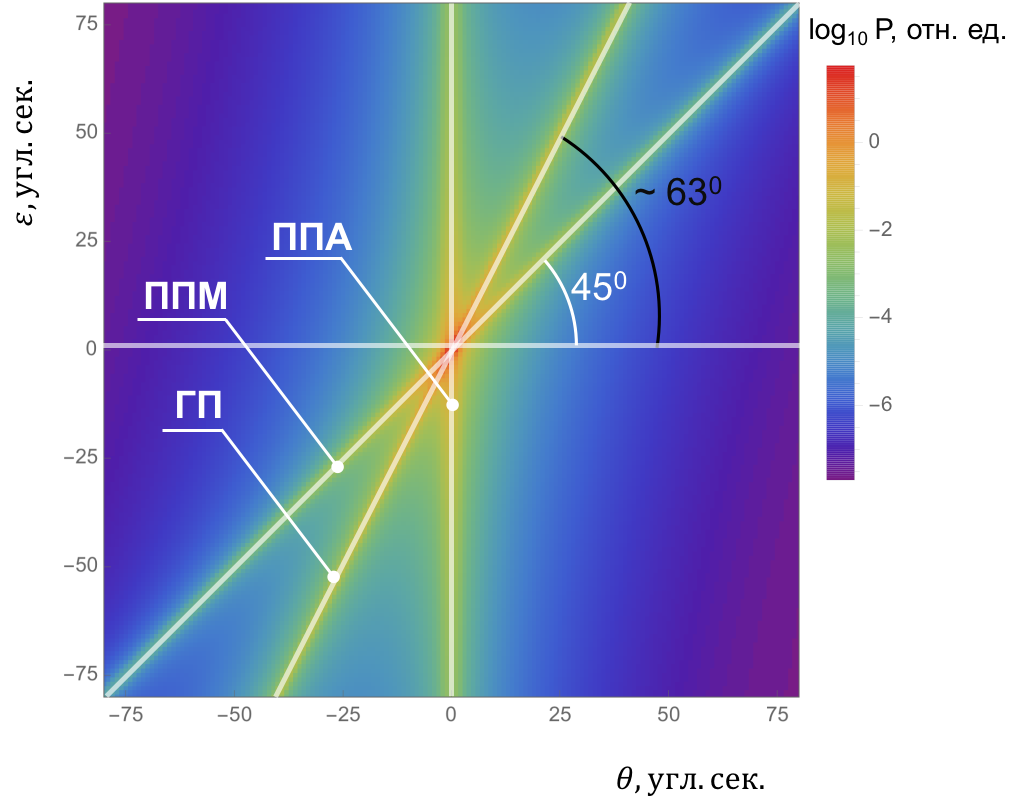
\includegraphics[width=0.6\textwidth]{images/triple_map_direct_space.png}
   \caption{Двумерная карта трехкристальной рентгеновской дифракции
   в координатах "отстройка образца $\theta$" -  "отстройка анализатора $\varepsilon$"}
   \label{ris:triple_map_direct_space}
 \end{figure}

Анализ показывает, что ГП находится под углом $63.4^o$, т.к. сканирование осуществляется вдоль $\varepsilon = 2 \theta$,
а $ \arctan \left(\frac{\varepsilon}{\theta} \right) = 63.4^o$. ППМ образует угол $45^o$, т.к. $\varepsilon = \theta$.
